% Autor: Leonhard Segger, Jannik Tim Zarnitz
% Datum: 2017-10-30
\documentclass[
% Papierformat
a4paper,
% Schriftgröße (beliebige Größen mit „fontsize=Xpt“)
12pt,
% Schreibt die Papiergröße korrekt ins Ausgabedokument
pagesize,
% Sprache für z.B. Babel
ngerman
]{scrartcl}

% Achtung: Die Reihenfolge der Pakete kann (leider) wichtig sein!
% Insbesondere sollten (so wie hier) babel, fontenc und inputenc (in dieser
% Reihenfolge) als Erstes und hyperref und cleveref (Reihenfolge auch hier
% beachten) als Letztes geladen werden!

\usepackage{tikz}
\usetikzlibrary{calc,patterns,angles,quotes} % loads some tikz extensions\usepackage{tikz}
\usetikzlibrary{babel}

% Silbentrennung etc.; Sprache wird durch Option bei \documentclass festgelegt
\usepackage{babel}
% Verwendung der Zeichentabelle T1 (Sonderzeichen etc.)
\usepackage[T1]{fontenc}
% Legt die Zeichenkodierung der Eingabedatei fest, z.B. UTF-8
\usepackage[utf8]{inputenc}
% Schriftart
\usepackage{lmodern}
% Zusätzliche Sonderzeichen
\usepackage{textcomp}

% Mathepaket (intlimits: Grenzen über/unter Integralzeichen)
\usepackage[intlimits]{amsmath}
% Ermöglicht die Nutzung von \SI{Zahl}{Einheit} u.a.
\usepackage{siunitx}
% Zum flexiblen Einbinden von Grafiken (\includegraphics)
\usepackage{graphicx}
% Abbildungen im Fließtext
\usepackage{wrapfig}
% Abbildungen nebeneinander (subfigure, subtable)
\usepackage{subcaption}
% Funktionen für Anführungszeichen
\usepackage{csquotes}
\MakeOuterQuote{"}
% Zitieren, Bibliografie
\usepackage{biblatex}


% Zur Darstellung von Webadressen
\usepackage{url}
%chemische Formeln
\usepackage[version=4]{mhchem}
% siunitx: Deutsche Ausgabe, Messfehler getrennt mit ± ausgeben
\usepackage{floatrow}
\floatsetup[table]{capposition=top}
\usepackage{float}
% Verlinkt Textstellen im PDF-Dokument
\usepackage[unicode]{hyperref}
% "Schlaue" Referenzen (nach hyperref laden!)
\usepackage{cleveref}
\sisetup{
	locale=DE,
	separate-uncertainty
}
%\bibliography{6Mi_M3_29-11-2017_References}
%TODO anpassen

\begin{document}
	
	\begin{titlepage}
		\centering
		{\scshape\LARGE Protokoll zu \par}
		\vspace{1cm}
		{\scshape\huge Einführung in rechnergestütztes Experimentieren \par}
		\vspace{3cm}
		
		{\large Jannik Tim Zarnitz (E-Mail: j\_zarn02@wwu.de) \par}
		{\large Leonhard Segger (E-Mail: l\_segg03@wwu.de) \par}
		\vfill
		
		in der Woche 03.09.2018 bis 06.09.2018\par
		betreut von\par
		{\large Dr. Jürgen Berkemeier}
		
		\vfill
		
		{\large \today\par}
	\end{titlepage}
	\tableofcontents
	\newpage

	\section{Tag 1} \label{Tag 1}
	
	\subsection{Aufbau einer Sinus- bzw. Bessel-Funktion}
	
	
	
	\subsection{Lissajous-Figuren}
	
	
	
	\section{Tag 2} \label{Tag 2}
	
	\subsection{Digitales Oszilloskop mit ExpressVI}
	Es wird ein Funktionsgenerator verwendet.
	Dessen Signal wird über einen Analog-Digital-Wandler durch den Computer erfasst.
	Zunächst wird das Signal in LabView mit dem entsprechenden ExpressVI verarbeitet.
	Das zugehörige Programm ist in \cref{fig_tag2_oszi_express_block} und die Frontplatte in \cref{fig_tag2_oszi_express_front} dargestellt.
	
	\begin{figure}[H]  
		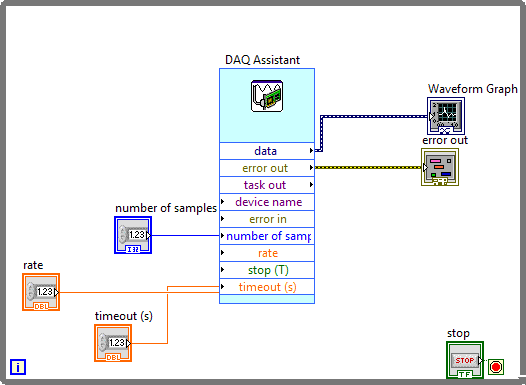
\includegraphics[width=1\textwidth]{EIRE2018Dateien/Tag2/expressVI_1d}
		\centering
		\caption{
			Einfaches Oszilloskop mithilfe des ExpressVIs zur Verarbeitung von Daten von Messgeräten.
		}
		\label{fig_tag2_oszi_express_block}
		\centering
	\end{figure}
	\begin{figure}[H]  
		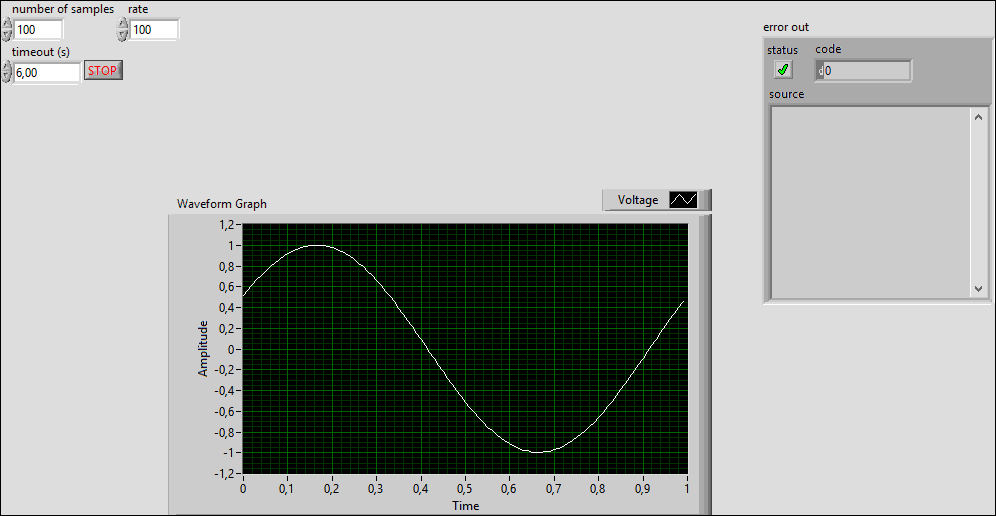
\includegraphics[width=1\textwidth]{EIRE2018Dateien/Tag2/expressVI_1p}
		\centering
		\caption{
			Frontplatte des einfachen Oszilloskop mithilfe des ExpressVIs zur Verarbeitung von Daten von Messgeräten. Dabei wurde durch den Funktionsgenerator ein sinusförmiges Signal ausgegeben.
		}
		\label{fig_tag2_oszi_express_front}
	\centering
	\end{figure}
	
	\subsection{Fouriertheorem} %kp, ob man so Theorie wiedergeben soll und ob man das mit Bindestrich schreibt.
	Gemäß des Fouriertheorems kann jede periodische Funktion als Fourierreihe bzw. Fourierintegral ausgedrückt werden.
	Dies ist nützlich bei der Zerlegung eines möglicherweise verrauschten Signals in seine Bestandteile.
	Das grundsätzliche Problem hierbei ist, dass Messprozesse immer zeitlich begrenzt ist, weshalb das Signal nicht bis in die positive und negative Unendlichkeit periodisch sein kann.
	%TODO und nun?
	
	\subsection{Abtasttheorem}
	%TODO kurze Zusammenfassung seiner Theorie-Sachen, hab ich auf Papier
	Um ein Signal abzutasten, werden im Analog-Digital-Wandler mithilfe einer Sample-and-Hold-Schaltung zeitlich diskrete Messungen durchgeführt.
	Dies lässt sich als Multiplikation des Signals mit einem Delta-Kamm ausdrücken.
	Dabei treten Summen- und Differenzfrequenzen der Abtastfrequenz (und deren Oberfrequenzen) und den Frequenzen im Signal auf.
	Im Frequenzraum ergibt sich hierdurch eine periodische Fortsetzung des Spektrums des ursprünglichen Signals, wobei die Periode der Abtastfrequenz entspricht, wobei auch die Differenzfrequenzen auftauchen. %TODO ist bissl unschön und man braucht vmtl. ein Bild. Ich weiß aber auch nicht, in wiefern man die Theorie noch mal aufrollen soll.
	Wenn die Abtastfrequenz hinreichend groß ist, kann man nun mithilfe eines Tiefpasses das Signal herausfiltern.
	Dazu muss sie allerdings größer als das Doppelte der höchsten im Signal auftretenden Frequenz sein, da sich ansonsten das Spektrum des Signals mit den Differenzfrequenzen der nächsten Periode überlagern.
	Dies bezeichnet man als Aliasing.
	
	
	\section{Tag 3} \label{Tag 3}
	%eig. zunächst Fertigstellung von Tag2 Teil 1
	
	\subsection{Digitales Oszilloskop ohne ExpressVI} % hier ist halt die Tagreihenfolge bissl gebrochen. Ich glaube, wir haben das an Tag 2 angefangen und Tag 3 beendet
	Das Oszilloskop-Programm von zuvor wird ersetzt durch eines, dass anstelle des ExpressVIs Konfiguration, Messung und Cleanup getrennt enthält.
	%TODO hier ansetzen
	
	\subsection{Leakage-Effekt und Fensterfunktion}
	
	\subsection{Aliasing}
	Um den Effekt des Aliasings absichtlich herbeizuführen, werden bei einer Abtastfrequenz von \SI{1000}{\hertz} zwei verschiedene Signale abgetastet.
	Da bei dieser Abtastfrequenz die höchste Frequenz im Signal kleiner als \SI{500}{\hertz} sein muss, ist hierbei zu erwarten, dass ein Signal von \SI{400}{\hertz} korrekt abgetastet wird, während eines mit \SI{600}{\hertz} falsch abgetastet wird.
	Das Spektrum des abgetasteten Signals bei diesen beiden Signalfrequenzen ist in \cref{fig_ali} dargestellt.
	
	\begin{figure}[H]
		\centering
		\begin{subfigure}[t]{0.5\textwidth}
			\centering
			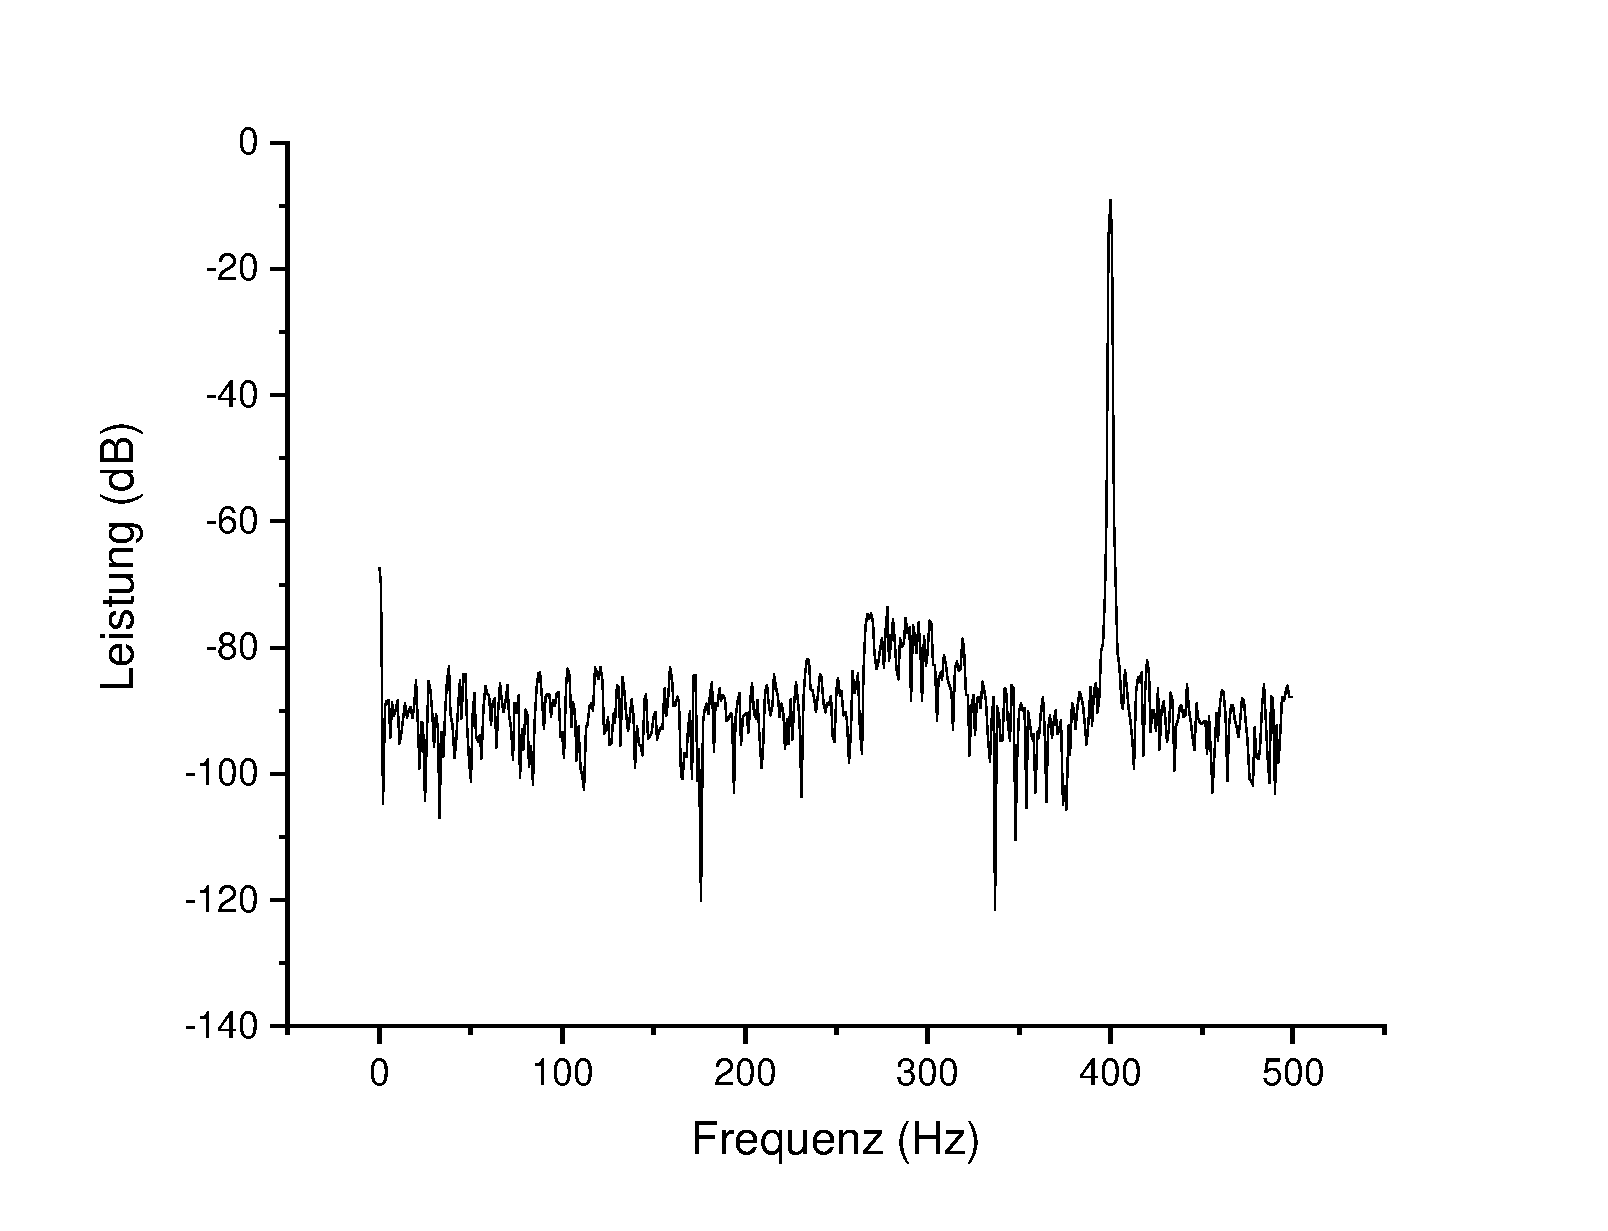
\includegraphics[width=1\textwidth]{Origin-Files/aliasing_abtast1000bei400sig}
			\caption{\SI{400}{\hertz}}
		\end{subfigure}%
		\begin{subfigure}[t]{0.5\textwidth}
			\centering
			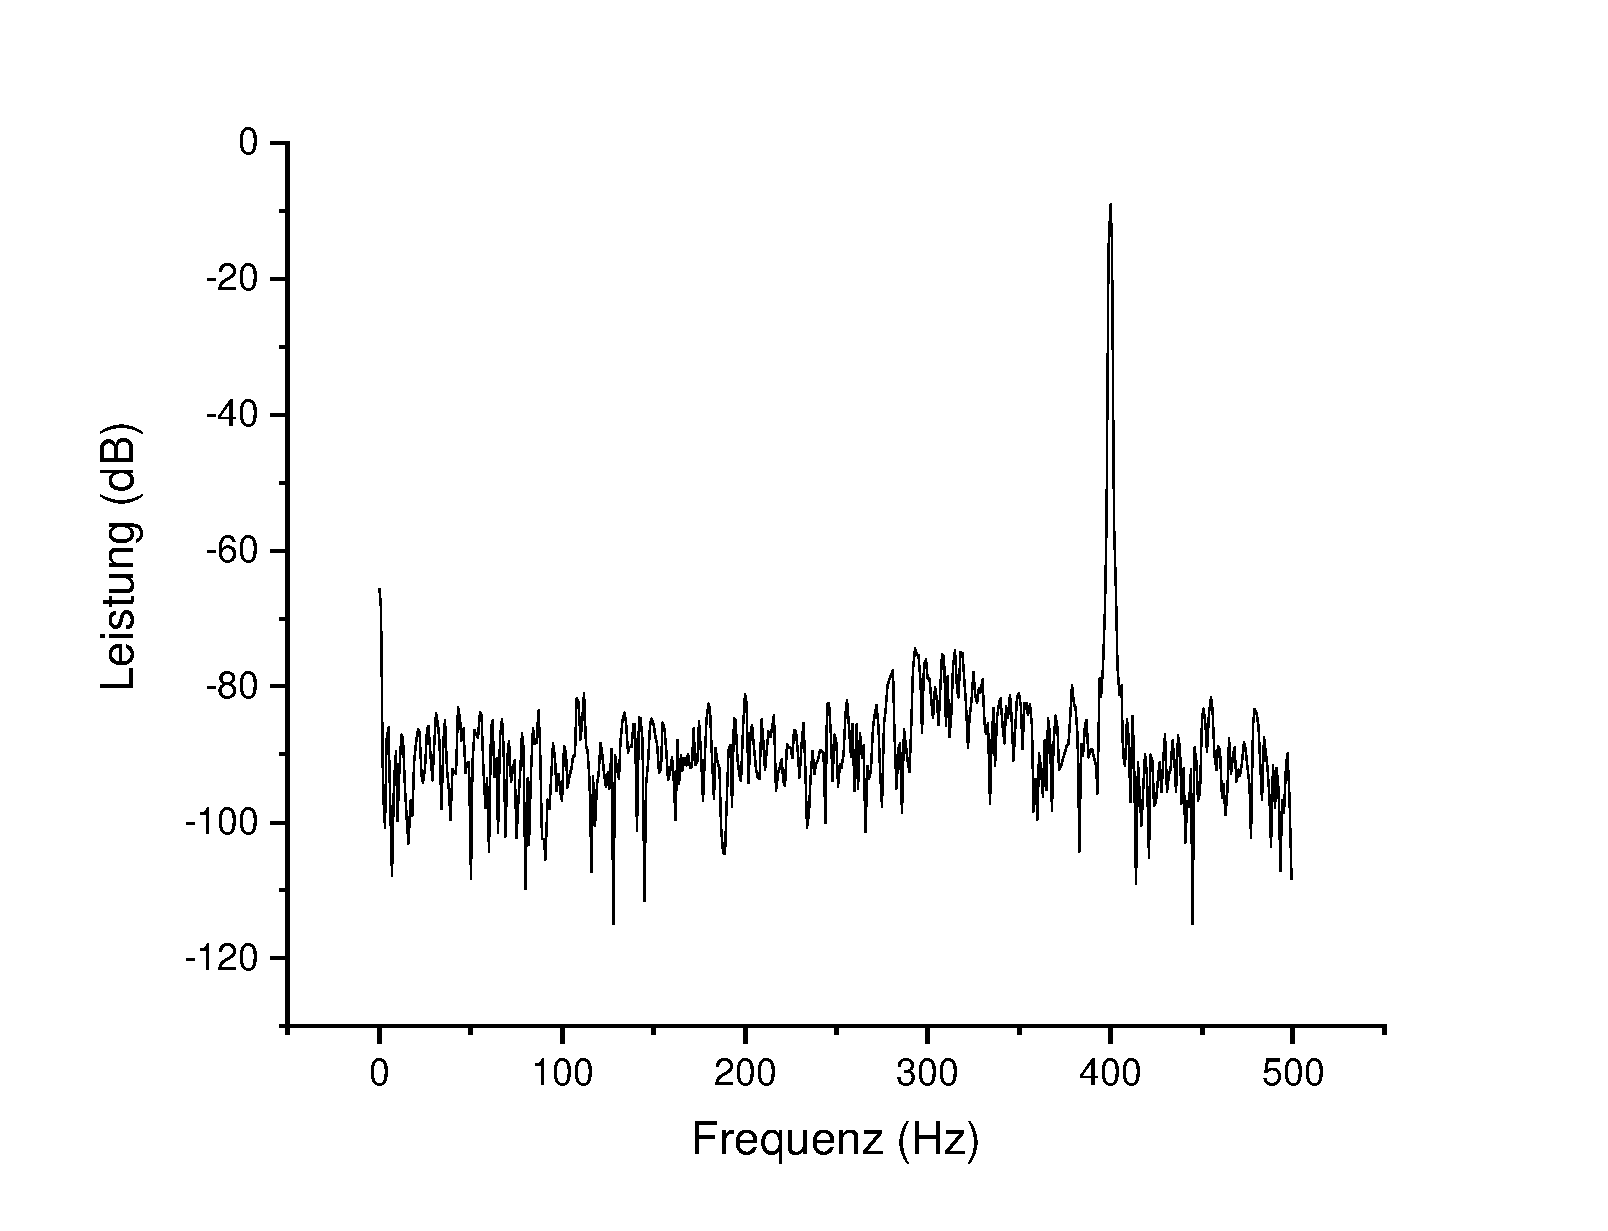
\includegraphics[width=1\textwidth]{Origin-Files/aliasing_abtast1000bei600sig}
			\caption{\SI{600}{\hertz}}
		\end{subfigure}
		\label{fig_ali}
		\caption{Mit einer Abtastfrequenz von \SI{1000}{\hertz} abgetastete Signale, deren Frequenz einmal \SI{400}{\hertz} und einmal \SI{600}{\hertz} beträgt, sodass einmal korrekt und einmal falsch abgetastet wird.}
		\centering
	\end{figure}
	
	Es fällt auf, dass sich zwischen diesen beiden Signalen kein Unterschied erkennen lässt.
	Dies liegt daran, dass bei einer Signalfrequenz von \SI{600}{\hertz} die eigentliche Signalfrequenz nicht mehr vom idealen Tiefpass übertragen wird, während die Differenzfrequenz von Abtastfrequenz und Signalfrequenz \SI{400}{\hertz} beträgt.
	Es ist an den beiden Signalen zu erkennen, dass sich ein falsch abgetastetes Signal nicht mehr von einem korrekt abgetasteten Signal bei der entsprechenden Differenzfrequenz unterscheiden lässt.
	Man stellt fest, dass man vor der Abtastung bereits wissen muss, welche Frequenzen im Signal vorkommen. 
	
	
	\subsection{Amplitudenmodulierte Signale}
	
	\subsubsection{Erzeugung}
	% + Ausgabe über Soundkarte
	
	\subsubsection{Demodulation}
	%Betrag, Quadrat
	
	\section{Tag 4} \label{Tag 4}
	
	\subsection{Demodulation eines AM-Signals mittels Trägerfrequenzmultiplikation}
	
	\subsection{Erzeugung eines phasen- bzw. frequenzmodulierten Signals}
	
	\subsection{Demodulation eines phasen- bzw. frequenzmodulierten Signals}
	
	\subsubsection{Erweiterte Demodulation mit Bandpass und zusätzlicher Integration des Signals}
	
	
	%\printbibliography
\end{document}
